\chapter{The Neutral apparatus}
\label{ch:chap2}

The Neutral apparatus has been one of the pioneering experiments for the trapping, cooling, and creation of quantum degenerate gases of neutral strontium \hl{BEC refs}. 
As such, there is a plethora of previous theses and publications which extensively outline the details for how to achieve these goals. \hl{refs}. 
In particular, we refer the reader to the PhD theses of previous Killian lab students: Francisco Camargo, Brian DeSalvo, Mi Yan, Pascal Mickelson, Natali Martinez de Escobar, and Sarah Nagel. 
Additionally, the PhD work of Simon Stellmer \cite{SimonStellmer2013} and review of strontium quantum degenerate gases are also highly recommended reading \cite{StellmerRev2013}.

Building upon this previous work, this chapter will forego an extensive review of the basic laser cooling techniques for strontium. 
We refer the reading to the extensive works listed above for a formal discussion of the theory behind laser cooling and trapping.
Instead, we will focus on the systems and processes which are crucial to the operation of the experiment with an emphasis on technical findings and changes which remain, as of yet, mostly undocumented.

Furthermore, it has been nearly a decade since the last broad apparatus overview \cite{MartinezdeEscolar2010} and the experiment has grown significantly in complexity in the intervening years.
Therefore, the goal of this chapter is to serve as a reference for future work and students. 
In this spirit, this chapter will be highly technical and provide an in-depth review of the operation and current status of the Neutral apparatus.
Where appropriate we will refer the reader to the relevant original thesis or published work.

This chapter will begin with a brief overview of our trapping procedure in order to contextualize the remaining sections focusing on the hardware including the vacuum system, various laser systems, and RF and electronics.
Furthermore, we will conclude with an outline of recent software implementations used to interface the digital world to the physical.
Detailed guides for this software can also be found in App. \ref{app:neuKLEIN}.

\section{Experimental procedure} \label{sec:trapping}

% Intro
Our experiments begin by cooling and trapping atomic strontium utilizing well-established atomic physics techniques \cite{Metcalf1999,Katori1999,Ido2000,Nagel2003,Mukaiyama2003a,Loftus2004,mmy09a,sth09a,Mickelson2010ja,Tey2010a,dym10a,stg10}. 
Fig. \;\ref{fig:energyLevels} shows the simplified energy level diagram employed in our cooling process. 
Once cooled, we typically obtain bulk samples in an optical dipole trap containing on the order of $10^6$ atoms at temperatures $<1\mu$K and densities between $10^{12} - 10^{15}\,$cm$^{-3}$ depending upon the isotope. 

The procedure outlined below is generally followed for trapping all isotopes of strontium with the major difference being timescales and laser frequencies.
Trapping of the bosonic isotopes of strontium is nearly identical across isotopes while fermionic $^{87}$Sr presents a greater challenge due to its high nuclear spin, $I=9/2$.
In short, due to the change in spin between the singlet and triplet series, there is a mismatch in the Zeeman shifts of the $^1S_0$ and $^3P_1$ states which leads to a change in sign of the Zeeman shift across the magnetic sublevels of the $^3P_1\,F=11/2$ hyperfine state of 87.
This sign change results in anti-trapped states causing atoms to be expelled from the MOT laser acting on the $^1S_0\,F=9/2\;\rightarrow\;^3P_1\,F=11/2$ transition.
The solution is then to add an additional laser addressing the $^1S_0\,F=9/2\;\rightarrow\;^3P_1\,F=9/2$ transition to randomize the $m_F$ populations in the $^1S_0$ ground state.
For a more thorough and detailed discussion of the relevant physics of trapping $^{87}$Sr in the red MOT, we refer the interested reader to the fermion portion of section 2.7.3 in the PhD thesis of Simon Stellmer \cite{SimonStellmer2013} and section 2.2.1 of Pascal Mikelson's PhD thesis \cite{Mickelson2010b}.

\noindent \rule{75pt}{0.5pt} \newline
The trapping process begins with vaporizing metallic strontium loaded in an oven heated to approximately 400 $^{\circ}$C. 
This strontium vapor escapes through thin collimating tubes to produce a partially collimated beam with a mean velocity of $\sim450$ m/s.
To aid in collimation, the atoms undergo a stage of transverse two dimensional optical molasses which is elongated and retro-reflected.
This helps increase the atom flux into the Zeeman slowing stage and we typically observe an approx. 7x improvement in trapped atom number with the 2D collimator versus without.
The majority of cooling is done using 461 nm light acting on the strongest dipole allowed transition between the $^1S_0\,\rightarrow\,^1P_1$ states.
The excited state lifetime of 5 ns ($\Gamma=30.5$MHz) and large energy separation between the states results in a hefty saturation intensity of 40.5 mW/cm$^2$ for this transition.
Therefore laser power on order of 100 mW are necessary to produce large optical forces and rapid cooling rates.

Once atoms have entered the magnetic field of the Zeeman slower, the highest velocity atoms begin to scatter photons from the Zeeman beam red detuned by approx. 16x the natural linewidth.
Large detunings help to eliminate unwanted photon scattering from the Zeeman beam once atoms have been sufficiently cooled and are accumulating in the MOT fields of the science chamber.
We note that while the principle functioning of the Zeeman slower only relies on the magnitude of the B-field along the solenoid, there is an interaction to be considered between the anti-Helmholtz MOT field and the decaying fringe fields of the Zeeman slower which can either lead to the fields adding or subtracting near the interface of the Zeeman and science chamber.
This subtle detail can have a large impact on trapping efficiency as we determined around 2014 when the current direction of the Neutral Zeeman slower was reversed from clockwise to anti-clockwise and we observed a 2x increase in trapped atom number at the conclusion of the blue MOT stage.

Once atoms have been slowed down to approx. 30 m/s we can capture using a magneto-optical trap (MOT) also working on the $^1S_0\,\rightarrow\,^3P_1$ transition. 
The optimal trapping frequency is tweaked for each isotope using our tunable sat. abs described in Sec. \hl{give ref}.
However, the typical detuning is approx $-3\Gamma/2 \approx -45$ MHz. 

MOT operation using this transition comes with the significant drawback that the Doppler temperature is relatively high at $T_D\approx1$ mK. 
The $J=0$ ground state of strontium also precludes the use of standard Sisyphus cooling techniques as there is only a single $m_J$ state available for bosonic strontium and far too many $m_F$ states in fermionic strontium.
Additionally, the $^1S_0\,\rightarrow\,^3P_1$ transition is not completely closed as shown in \;\ref{fig:energyLevels} resulting in population of the long-lived $^3P_2$ state. 
Fortunately, both of these obstacles are easily overcome.

The leak to the $^3P_2$ state results in population of magnetically trappable low-field seeking $m_j$ states. 
These atoms are trapped by the anti-Helmholtz field of the MOT and are dark to the 461 nm light \hl{natali refs (I think) [78, 79, 80, 65]}.
This allows us to take advantage of the long lifetime of the metastable $^3P_2$ state and accumulate a large number of atoms which can then be repumped back down to the $^1S_0$ ground state.
One drawback to this process is the long timescale required for a significant number of atoms to accumulate in the magnetic trap compared to the MOT.
However, the lifetime of the magnetic trap is typically limited by background pressure (approx. 15 - 25s) and therefore the maximum number of atoms which can be held by the magnetic trap is much greater than in the MOT. \hl{plots of loading between MOT and magnetic trap?}
On average, an atom will fall into the $^3P2$ state after scattering $10^5$ photons from the $^1S_0\,\rightarrow\,^3P_1$ transition and even then, only 2 out of 5 of the magnetic sub-levels are trappable.
Repumping is achieved via a 481 nm transition along the $(5s5p)^3P_2\,\rightarrow\,(5p^2)^3P2$ transition for approx. 50ms.
During the repumping exposure we continue to illuminate the cloud with 461 nm light but reduce the light intensity by an order of magnitude.
We refer to this stage as the "cold" blue MOT and find that reduction of the intensity, while maintaining consistent laser detuning, increases the transfer efficiency into the red MOT stage.
\footnote{We have explored ramping the laser intensity closer to atomic resonance as we expected reduced intensity at farther red-detuning to result in a weakened trapping force.
However, we did not find any improvement with the added complexity of varying the blue laser frequency during this stage.}

Once the atoms have been returned to the ground state, we begin a second MOT stage using the narrow intercombination transition $^1S_0\,\rightarrow\,^3P_1$ to cool below 1 mK.
The $(5s5p)^3P_1$ state has a reasonably long lifetime of 21 $\mu$s ($\Gamma/2\pi=7.5$ kHz).
This long lifetime and near-IR wavelength transition has a Doppler limit of approx. \hl{450 nK??} and a recoil temperature of \hl{900 nK??}.
The narrow line MOT operates in a different regime compared to typical dipole allowed MOTs as the narrow linewidth means that only a thin shell of the atomic cloud is resonant at a given laser detuning and magnetic field value.
We can simulate the behavior of a broad transition by frequency modulating the 689 nm light using voltage controlled RF sources coupled to the light via an acouto-optic modulator (AOM). 
Additionally, we begin the narrow line cooling with the center frequency, amplitude of modulation, and laser intensity at large values in order to trap the initially hotter atoms from the blue MOT stage. 
As cooling with the 689 nm light becomes effective, we dynamically vary these three parameters along with the magnetic field gradient in order to cool the entire sample.
Ultimately, the MOT is reduced to single frequency operation at low laser intensity to and we achieve final temperatures between 1 - 2 $\mu$K after 400 ms of cooling.

During the last 50 - 100 ms of the 689 MOT (typically during single frequency operation) we additionally overlap the high intensity 1064 nm optical dipole trap (ODT).
The red MOT can then cool atoms into the typically 10 $\mu$K deep ODT with relative ease with transfer efficiencies as high as 75\%. 
Next, we extinguish the red MOT and allow a period of free evaporation for the sample to equilibrate in the ODT before beginning forced evaporative cooling to produce our final sample of ultracold or quantum degenerate gas.

The end of the evaporation typically marks the beginning of the experimental phase and the divergence of our protocol into the specific procedures necessary. 
These may include ramping or pulsing on lattice beams, exciting a collective mode, probing the gas with PAS laser, shelving, etc. 
Once we have completed the experimental phase, we measure the cloud characteristics via absorption imaging along the $^1S_0\,\rightarrow\,^1P_1$ transition. 
Typically we perform absorption imaging following a time-of-flight so as to measure both the atom number and temperature at the time of release. 
However, this is not strictly necessary and certain experiments may result in low atomic densities which are not amenable to a time-of-flight due to their low optical depth.

\subsection{Characteristic performance} \label{sec:benchmark_trapping}

The following subsections outline typical trapping parameters and performance for each isotope. Note, that while we have demonstrated the ability to dual trap 84 and 87, full characterization and optimization of this process is currently the subject of investigation.

\paragraph{$^{84}$Sr} \label{sec:84_trapping}

Timing diagram
	Blue MOT
	Repump
	Broadband red MOT
	Single Freq red MOT
	IR loading
	Evaporation: typically around 1 to 7s
	Time of flight
	Imaging
Typical settings table
Performance table

\paragraph{$^{86}$Sr} \label{sec:86_trapping}

\paragraph{$^{87}$Sr} \label{sec:87_trapping}


Remember the switch to single frequency

What about values for the experiments?

\hl{would like to put a timing diagram here showing a typical timing sequence for 84, 86, and 87}

Where the heck does that calibration for the MOT coils come from??

\paragraph{Daily statistics} \label{sec:dailyStats}
The following is a table of daily measurements and selected values for evaluating the long-term performance of the apparatus.
This partial list is shown here to document those parameters which should be recorded on days the apparatus will performing trapping.
Some columns do not contain data as the requisite measurements have evolved over the years\footnote{The full spreadsheet is currently located at \texttt{KillianDrobo:\textbackslash Neutral\textbackslash Daily Statistics.xlsx}}.

\section{Vacuum system and atom source} \label{sec:vac}

\paragraph{Overview}
	
The Neutral apparatus is built around a custom stainless steel chamber positioned above the table to facilitate optical access. Typical pressures are in the ultrahigh vacuum regime, $<1\times10^{-10}$ torr. 
Details on the original construction can be found in Natali (App. A.10) and Pascal's theses \cite{MartinezdeEscolar2010,Mickelson2010b}. The master's of Francisco Camargo \cite{Camargo2015} outlines the construction of the similar Rydberg apparatus. This more recent apparatus has benefited from the many lessons learned during the early life of the Neutral experiment.
\newline

% Complete assembly
\noindent The vacuum system can be decomposed into several subcomponents, namely
\begin{enumerate}
\item Atom source (assembly of atom oven housed within the source chamber)
\item 2D collimator
\item Zeeman slower
\item Science chamber
\item Cryo tower
\end{enumerate}
Figure \ref{fig:vacuumSystem} shows a complete overview of these assemblies which form our vacuum system.
	\begin{figure} 
		\centerline{
		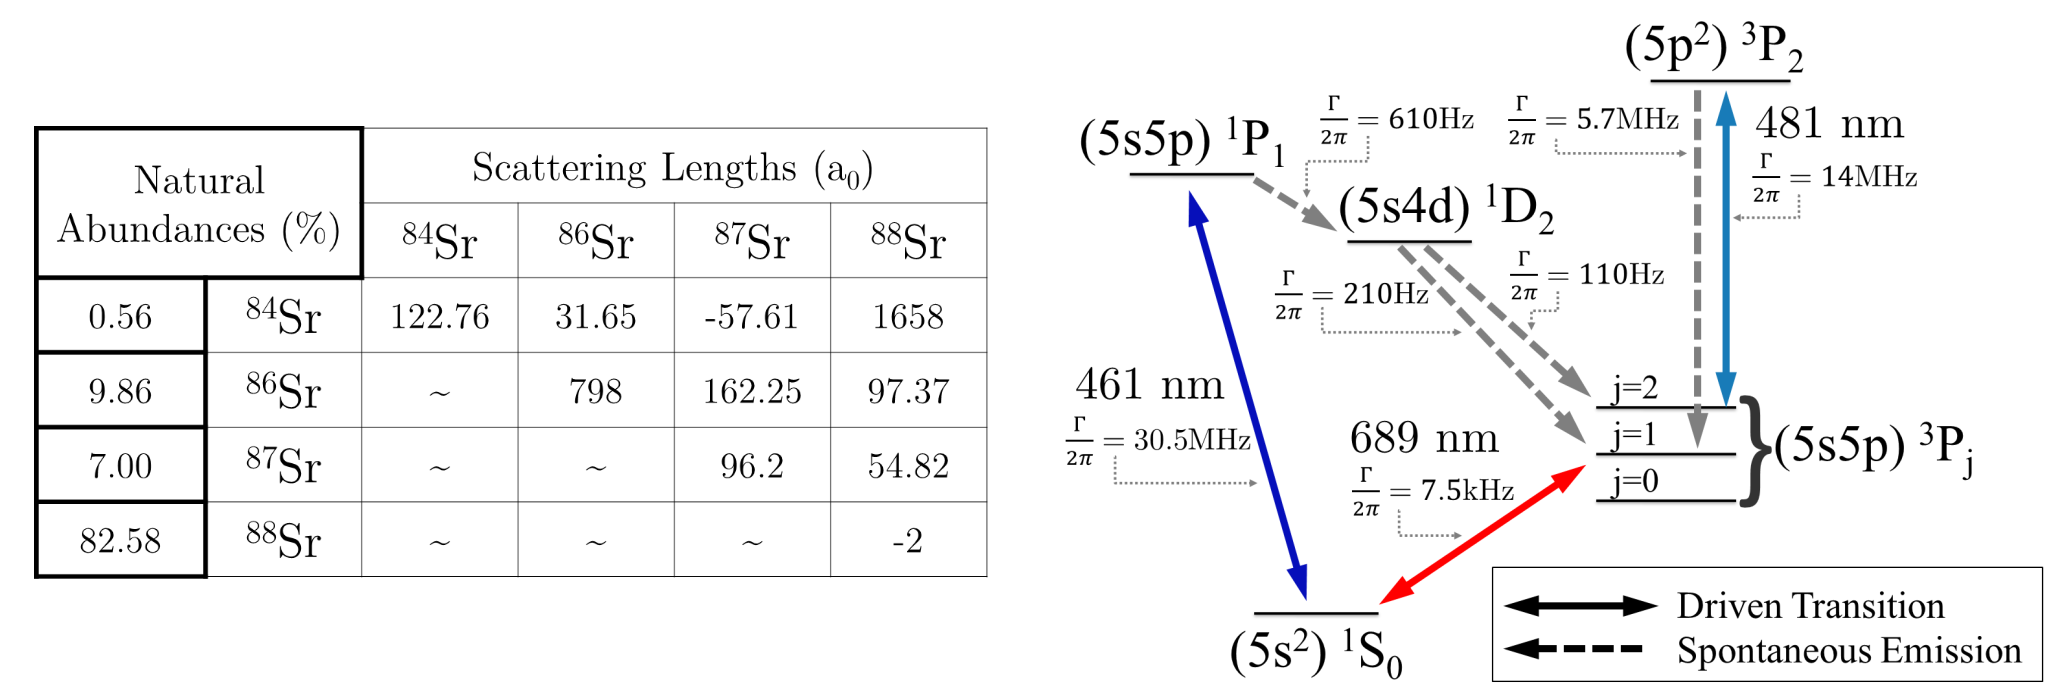
\includegraphics[angle=90,origin=c,height=0.6\textheight]{strontium_properties.pdf}}
		\caption{Complete Neutral apparatus vacuum system}
		\label{fig:vacuumSystem}
	\end{figure}
Figures \ref{fig:sourceSideView} - \ref{fig:cryoTower} also show various views of the atom source, 2D collimator, and cryo tower assemblies. Note the red markers and green arrows denote the positions of heater bands and thermo-couples respectively. For more information please see App. \ref{app:breakingVacuum}.
	\begin{figure} 
		\centerline{
		\includegraphics[height=0.4\textheight]{vacuum_source_assembly.png}}
		\caption{Source assembly - side view}
		\label{fig:sourceSideView}
	\end{figure}
	
	\begin{figure} 
		\centerline{
		\includegraphics[height=0.4\textheight]{vacuum_source_rearView.png}}
		\caption{Source assembly - rear view}
		\label{fig:sourceRearView}
	\end{figure}
	
	\begin{figure} 
		\centerline{
		\includegraphics[height=0.5\textheight]{vacuum_2D_collimator.png}}
		\caption{2D collimator assembly}
		\label{fig:assembly_2Dcoll}
	\end{figure}
	
	\begin{figure} 
		\centerline{
		\includegraphics[width=1.25\textwidth]{vacuum_tower.png}}
		\caption{Cryo tower assembly}
		\label{fig:cryoTower}
	\end{figure}
From left to right, the system starts with an oven source based around a custom nozzle design which uses a rod heater to vaporize elemental strontium.
Next, there is a 6 way tee used for the optical molasses step which we refer to as the 2D collimator. 
From here atoms pass through a narrow differential pumping tube and into the entry port of the Zeeman slower where a majority of the laser cooling takes places. 
Following the Zeeman slower, atoms enter the science chamber where a plethora of lasers are used to manipulate and probe their behavior.
Chief among these are the MOT sequences and the high intensity far off-resonant optical dipole traps used for the final stage of confinement.
Lastly, the body of the science chamber is supported by the cryo tower which houses a titanium sublimation catridge (model: Varian 916-0061 series) and is the entry point for the Zeeman laser.
It is worth explicitly noting that this Zeeman window is necessarily directly opposite the atomic source and therefore is subject to a flux of hot atomic strontium which will eventually coat the vacuum side. A brief note on a possible solution to this problem is explored at the end of this section.

While the source and science chamber have remained largely unchanged since the publication of Natali's thesis, several key improvements and events have occurred over the last few years\footnote{As of April 2019, the most up to date CAD drawing for the Neutral apparatus is located at \texttt{KillianDrobo:\textbackslash Neutral\textbackslash Laboratory Systems\textbackslash Vacuum Chamber\textbackslash Neutral Chamber\textbackslash 2017.12.26\_strontiumvacuum35\_latticetable.dwg}. Additionally, please consult the README file located in this folder for further information.}.
These differences will be the subject of our discussion in the latter part of this section.


% Orientation of lasers to chamber 
Fig \hl{something} shows a closer view of the science chamber and defines a coordinate system as well as directional labels used throughout this thesis. 
We will use this reference when illustrating the orientation of various lasers through the science chamber to help the reader.
Furthermore, table \hl{something} lists the ports and their respective windows as of April 2019.
This table builds from table A.9 in Natali's thesis \cite{MartinezdeEscolar2010}.

The original drawings of these components can be found in App. A.10 of \cite{MartinezdeEscolar2010} along with detailed information of the window and ion gauge placements. 

\paragraph{Recent changes}
\subparagraph{Addition of platform:}
During the push to produce quantum degeneracy of strontium it was determined that different geometries of traps were necessary to achieve efficient forced evaporation. 
To this end, the task of redesigning the optical dipole traps was undertaken by Ying Huang and is detailed in her master's thesis \cite{Huang2013}. 
A raised platform was designed and built around the chamber to facilitate this project.
Unfortunately, while a major portion of this platform design is available in the main apparatus CAD file, the platform opposite of the oven is not documented.
Nor is there a complete assembly drawing incorporating the chamber and platform, which may confound future efforts to build around the chamber as more complexity is introduced. 

Currently, nearly every optical probe is launched from this raised platform.
This includes the 1064 nm bulk optical dipole trap and the 532 nm optical lattice, both of which are outlined below. 
During installation of the free space optical lattice we observed heating and hypothesized that relative movement of the platform and chamber may be a cause.
Supporting struts were then added beneath the chamber in an attempt to secure it to the platform around 2016.
However, the extreme sensitivity of cold atoms and occasional observation of shot to shot fluctuations persists the concern of relative movement between non-rigid components.

These concerns were reinforced when we observed increased stability once a partial cover was added over the platform optics for the optical dipole and lattice traps. 
Initially meant as an optical safety measure to enclose the high power beams, we noticed a marked decrease in the shot to shot fluctuations of the cloud position after a time of flight.
With further testing we were able to attribute the increased stability to a mitigation of air currents caused by close proximity of the platform optics to the ventilation system meant to thwart dust accumulation inside the experimental enclosure.

% Running out of strontium
\subparagraph{Running out of strontium:}
In the winter of 2017 the neutral apparatus had been under vacuum for approx 8 years when suddenly we were no longer able to trap a significant number of atoms \footnote{It is was expected any trapping loss due to low strontium would be gradual and we were not able to determine the cause of the abrupt behavior.}.
After extensive testing, we hypothesized that we had run out of elemental strontium within the atomic source.
This led us to break vacuum, reload strontium, and perform a light bakeout procedure to reestablish the requisite ultrahigh vacuum for experiments.
Details of this bakeout procedure can be found in App. \ref{app:breakingVacuum}. 
Through this process we confirmed our hypothesis that lack of strontium was the cause of the issue. 
Figure \ref{fig:2d_coll_flourescence} shows the atom beam fluorescence after refilling the oven.
This image was taken while using the Zeeman laser to cause photon scattering and looking down the 2D collimator.
	\begin{figure}
		\centerline{
		\includegraphics[height=0.5\textheight]{vacuum_IMG_20171103_184vacuum_230.jpg}}
		\caption{Typical fluorescence of Zeeman beam looking down 2D collimator}{This view is found using a 2 in mirror aligned along the path of the first pass of the 2D collimator (near mirror 3 in the diagram), looking down the collimator tube. While looking at this angle, we are able to see the Zeeman beam move across the atom column when moving the last turning mirror. Reduction in this fluorescence signal from that shown was the primary indicator of lack of strontium in the source.}
		\label{fig:2d_coll_flourescence}
	\end{figure}  
Prior to this event the Neutral apparatus enjoyed lifetimes of approx. 25s as measured by background lifetimes measurements within the IR optical dipole trap. 
Approximately a year after restoring vacuum we have measured lifetimes on the order of 15s, the cause of the discrepancy is not rigorously known. \hl{verify time, plot maybe?}

During the process of breaking vacuum we attempted several upgrades to the apparatus including adding a gate valve between the cryo tower and the Zeeman window as well as redesigning the atom nozzle source to incorporate a fixed heat shield around the heating element. 
Details of the nozzle design can also be found in App. \ref{app:breakingVacuum}.
Unfortunately, long lead times from vendors and a mistake in the nozzle construction led us to move forward and re-establish vacuum without these upgrades in place.

Finally, after removing the atom oven to replace strontium, we placed a temporary viewport to facilitate alignment of the Zeeman beam through the length of the vacuum system. 
While aligning we observed an unexpected partial occlusion of the Zeeman beam and upon further investigation learned that the differential pumping tube is noticeably not parallel to the atom trajectory.
We were not able to determine the severity of the misalignment since the tube is not easily accessible and replacement is problematic as the tube is attached to a copper gasket held between flanges connecting the atom source chamber and the 6-way tee of the 2D collimator. 
The main readily measurable symptom is the occlusion of the Zeeman beam which with an input power of approx. 120 mW before expansion optics and entering the chamber, only measures approx. 60 mW of transmitted power through the length of the vacuum system. 
A solution to bend the soft copper with a rod was proposed but abandoned due to concerns of cracking the thin copper.
As adequate repair of the tube necessitates a drastic and practically infeasible deconstruction of the vacuum system our goal here is to document the issue for future students.
It is currently hypothesized that this problem is the primary cause of the much longer load times needed in the Neutral apparatus compared to the newly designed Rydberg machine.

\paragraph{Clarifications from de Escobar thesis}

collimate 
% cryo tower
\subparagraph{HV version 1 \& 2:}
As a point of clarification, Natali's thesis \cite{MartinezdeEscolar2010} presents two versions of the HV chamber in figures A.42 - A.47 while referencing that the original construction proceeded with version 1. 
However, version 2 (the cryo tower) was installed around 2011 and is currently in use. Version 2 is shown in Fig. \ref{fig:cryoTower} and details are available in the apparatus CAD drawing.

\subparagraph{Collimating array in nozzle:}
% hypodermic needle nozzle
Once more, Natali's thesis refers to the installation of an improved nozzle design incorporating an array of collimating tubes constructed from 2$\mu$ hypodermic needles (model: \hl{find}). 
Modeling and construction of this design was done by Anton Mazurenko, \cite{Mazurenko2010}, with the goal of improving the angular discrimination of the oven assembly to produce a more highly collimated beam of atoms.
Figure \ref{fig:2010_nozzle} shows the improved nozzle design \footnote{For reference, this nozzle design is labeled "new nozzle summer 2010" in the apparatus CAD file to distinguish it from the other nozzle drawings also present.}.
	\begin{figure}
		\centerline{
		\includegraphics[height=0.4\textheight]{vacuum_nozzle.jpg}}
		\caption{Atom oven and nozzle construction}{a) The nozzle through which vaporized strontium enters the experiment. Here we see the array of collimating tubes behind which solid strontium is packed. b) The complete oven construction which houses the cartridge heater and the nozzle at the tip.}
		\label{fig:2010_nozzle}
	\end{figure}
The original assembly of this oven also incorporated a heat shield that would insert over the construction shown in Fig. \ref{fig:2010_nozzle}b) but was ultimately abandoned since there was no way to fasten it to the flange which led the shield to fall off.
We hypothesized that lack of a heat shield led to uneven distribution of the thermal energy throughout the oven.
Therefore, fastening of the heat shield to the base flange was the primary goal of the redesign undertaken in late 2017 and further details can be found in App. \ref{app:breakingVacuum}.  
 
\paragraph{Ablating strontium off window} \label{p:ablatingSr}
While not directly related to any experiment or typical procedure, this sub-section summarizes a brief side project of using a pulsed 532 nm Verdi to ablate strontium from a vacuum window.
As discussed previously, a common problem faced by strontium experiments is the accumulation of strontium on the Zeeman entry port. 
These deposits may then act as a partial mirror leading to attentuation of the crucially important Zeeman beam. 
It was shared through private communication with professor Killian that pulsed 532 nm light (such as from a q-locked Verdi system used in the Plasma laboratory) might vaporize the strontium off the window and restore any loss in power. 
Using a test apparatus we were able to verify that indeed we could ablate the strontium off of a coated window, as shown in figure \ref{fig:ablating_strontium}.
	\begin{figure}
		\centerline{
		\includegraphics[width=0.8\textwidth]{vacuum_ablated_sr2.jpg}}
		\caption{Ablating strontium coating from window}{Comparison of the before (left) and after (right) when using a pulsed 532 nm Verdi to ablate strontium. The residue visible in the after image we believe to be caused by too high of an energy pulse which was reduced as we moved towards the center of the window.}
		\label{fig:ablating_strontium}
	\end{figure}
This promising test led us to install an optical traversal port, shown in figure, connecting the Plasma and Neutral labs. 
Unfortunately, while flashing the Verdi on a small section of the Neutral Zeeman window we found that the energy needed to ablate the strontium was accompanied by deformation of the optical surface.
We discontinued the ablation upon observing this behavior as we did not want to distort the optical beam front of the Zeeman front.
Instead, we replaced the window upon breaking vacuum as previously noted.
Additionally, in an effort to mitigate the time the window was exposed to the hot strontium beam, we installed a small servo motor to drive the atom shutter valve and integrated this mechanism into the experimental runtime. 
This allows the shutter to only be open during the times that we are actively trapping atoms. 
Details of the servo motor trigger integration into the neuKLEIN control system are available in App \hl{somewhere}.

\section{Laser systems}\label{sec:laser_systems}

The heart of any atomic physics experiment are the laser systems which are the basis for laser cooling and various probes.
Our lab has transitioned to mainly using diode lasers and we rely heavily upon the use of injection locked master - slave setups. \hl{ref}
Below we will outline the specifics of our light generation systems.
In particular, future experiments on the Neutral apparatus aim to explore quantum magnetism using strontium 87 and as such we will emphasize several key changes which have been made to the 461 locking and 689 trapping systems.

\subsection{Wideband cooling stage: 461 nm}
\label{ssec:461sys}

\subsubsection{Overview}
As discussed in the experimental overview, the majority of our laser cooling is done using 461 nm light. 
We generate and control these photons by amplifying and frequency doubling 922 nm light from a master ECDL diode laser. 
Fig.\ref{fig:461blockSys} shows an overview of how we generate the 461 nm light. 
We will cover the 922 master, Zeeman sub-system, and MOT sub-systems in detail below.
As we can see from the figure, the MOT sub-system is the basis for many different components of the overall 461 generation.
These separate systems will also be addressed in the MOT sub-system section below.
	\begin{figure}
		\centerline{
		\includegraphics[width=\textwidth]{461_sys_overview.jpg}}
		\caption{461 nm light generation system}{a) Block diagram of showing the relations of the various systems, AOMs, and frequencies used to lock the system for 461 nm trapping and spectroscopy. See Table \ref{tab:461AOM} for information on the AOMs. b) Relative frequencies at various stages of the 461 system.}
		\label{fig:461blockSys}
	\end{figure} 

In conjunction with the block diagram, Table \ref{tab:461AOM} shows the details of the frequency shifts and AOMs. 
The position of these AOMs is represented by the numbered black circles while the labeled red squares define the various system frequencies.
These frequency relations are schematically represented in Fig. \ref{fig:461blockSys}b) and can be recreated via Eq. \ref{eq:461freqs}.
Table \ref{tab:461AOM} defines the shift variables used in these equations.
\begin{landscape}
\begin{table}[]
\centering
\begin{tabular}{@{}|l|c|l|c|c|l|l|l|@{}}
\toprule
\multicolumn{1}{|c|}{\textbf{Label}} & \textbf{Ind.} & \multicolumn{1}{c|}{\textbf{System}} & \textbf{\begin{tabular}[c]{@{}c@{}}Shift\\ variable\end{tabular}} & \textbf{\begin{tabular}[c]{@{}c@{}}Nominal \\ Freq. {[}MHz{]}\end{tabular}} & \multicolumn{1}{c|}{\textbf{Freq. Source}} & \multicolumn{1}{c|}{\textbf{Freq. control}} & \multicolumn{1}{c|}{\textbf{AOM Model}} \\ \midrule
Zeeman & 1 & 922 master & $\delta_{zeeman}$ & -252.4 & \begin{tabular}[c]{@{}l@{}}Mini Circuits\\ ZOS-300\end{tabular} & Static voltage & \begin{tabular}[c]{@{}l@{}}Crystal Tech. \\ 3200-1113\end{tabular} \\ \midrule
Blue MOT & 2 & MOT & $\delta_{bMOT}$ & +35.5 & \begin{tabular}[c]{@{}l@{}}Mini Circuits\\ ZOS-50\end{tabular} & Static voltage & \begin{tabular}[c]{@{}l@{}}IntraAction \\ AOM-402A1\end{tabular} \\ \midrule
Image 2 & 3 & \begin{tabular}[c]{@{}l@{}}Abs. imaging\\ \& Blow away\end{tabular} & $\delta_{img2}$ & +75.6 & \begin{tabular}[c]{@{}l@{}}Mini Circuits\\ ZOS-75+\end{tabular} & Static voltage & \begin{tabular}[c]{@{}l@{}}IntraAction \\ ATM-1001A1\end{tabular} \\ \midrule
Image 1 & 4 & Abs. imaging & $\delta_{img1}$ & -52.8 & \begin{tabular}[c]{@{}l@{}}Mini Circuits \\ ZOS-150\end{tabular} & Static voltage & \begin{tabular}[c]{@{}l@{}}IntraAction \\ AOM-602A1\end{tabular} \\ \midrule
Blow away pulser & 5 & Blow away & $\delta_{BA}$ & -80 & \begin{tabular}[c]{@{}l@{}}IntraAction \\ ME-801T7\end{tabular} & Internal synth. & \begin{tabular}[c]{@{}l@{}}IntraAction \\ ATM-802DA1\end{tabular} \\ \midrule
Sat. abs. shifter & 6 & Sat. abs & $\delta_{SA}$ & +317.3 & \begin{tabular}[c]{@{}l@{}}Mini Circuits \\ ZOS-400+\end{tabular} & Static voltage & \begin{tabular}[c]{@{}l@{}}Crystal Tech. \\ 3200-141\end{tabular} \\ \bottomrule
\end{tabular}
\caption{461 nm systen AOM details}{Ind. refers to the number black circles in Fig. \ref{fig:461blockSys}. The sign of the nominal freq. indicates the AOM order}
\label{tab:461AOM}
\end{table}
\end{landscape}

\begin{align} \label{eq:461freqs}
	&f_{\text{motSys}}  = 2f_{922}          & &f_{\text{zeeSys}}  = 2(f_{922} + \delta_{\text{zeeman}}) \nonumber \\
	&f_{\text{2dColl}}  = f_{\text{motSys}} & &f_{\text{bMOT}}    = f_{\text{motSys}} + \delta_{\text{bMOT}} \nonumber \\
	&f_{\text{img}}     = f_{\text{motSys}} + \delta_{\text{img2}} + \delta_{\text{img1}} & &f_{\text{SA}} = f_{\text{motSys}} + \delta_{\text{SA}} \nonumber \\
	&f_{\text{BA}}      = f_{\text{motSys}} + \delta_{\text{img2}} + \delta_{\text{BA}}
\end{align}

Overall frequency control, $f_{922}$, is determined via the magnetically tunable saturated absorption cell.
This magnetic tunability to control the 461 nm light frequency is well documented in section 2.2.1 of Natali's thesis \cite{MartinezdeEscolar2010} and section 2.1.1 of Pascal's thesis \cite{Mickelson2010b}.
A more recent undergraduate project explored optimizations of this scheme for the Rydberg apparatus as well \cite{MichaelViray2014}.

\subsubsection{922 nm master}
The master 922 laser is derived from Sacher Lynx 922 nm IR diode laser in a Littrow ECDL configuration.
Fig. \hl{something}, shows a simplified optical schematic and Table \hl{some} gives typical running characteristics.
Starting at the master output, the beam is shaped and sent through a two optical isolator before it is coupled into an optical fiber.
The fiber output immediately goes through an AOM which detunes the diffracted order by approx. 250 MHz.
The diffracted and zeroth order are then separated with the unshifted beam sent towards the MOT generation subsystem and the shifted light towards the Zeeman subsystem.
We find it necessary to include dual isolators in front of the master laser and have found that inadequate alignment of these isolators can lead to significant instability in the frequency stability of the master which in turn leads the cavities to be unable to maintain a lock.

Light out of the 922 master has sidebands added via a high bandwidth AC coupled current modulation directly to the laser diode 
\footnote{This direct coupling means the RF must be turned on prior to enabling the DC current. 
Conversely, the DC current should be disabled before turning off the RF source. 
Failure to follow this order may result in destruction of the laser diode.}.
The doubling cavities of the MOT and Zeeman sub-systems are length stabilized via these sidebands using the Pound-Drever-Hall (PDH) technique \hl{refs}.
Currently, the RF source in use is a PTS 160 from Programmed Test Sources with an output power of 12 dbm and frequency of 39.55 MHz.
This RF is sent to a 3-way power splitter (model: Mini Circuits ZSC-3-1) which sends roughly a third of the power ($\sim$ 4 dbm) to each of the MOT and Zeeman PDH mixers for demodulation. 
The remaining third is attentuated by 3db before coupling directly to the laser diode.

In order to frequency stabilize the 922 nm, light from the MOT sub-system is used to interrogate a strontium heat pipe via frequency modulated Doppler-free saturated absorption from which an error signal of the $^1S_0\,\rightarrow\,^1P_1$ transition is derived.
This error signal is sent into a homemade integrator circuit with a fast feedback path controlling the 922 nm diode current and a super low-bandwidth\footnote{This super low-bandwidth lock is based on an Arduino PID controller with a low time constant and was built by Josh Hill.
We refer the interested reader to Josh's forthcoming thesis for details of this general purpose slow lock.} 
path controlling for long term frequency drifts via the ECDL's internal PZT.
We found that addition of this slow lock has significantly improved the continuous lock time of the 461 system. 
When enabled the experiment may stay locked for upwards of 24 hours at a time. 
As expected, such an increase in stability has greatly improved our ability to take data over long periods.
A block diagram of this feedback path is shown in Fig. \ref{fig:922freqLock}.
	\begin{figure}
		\centerline{
		\includegraphics[width=\textwidth]{922_locking_block diagram.jpg}}
		\caption{922 nm frequency stabilization block diagram}{}
		\label{fig:922freqLock}
	\end{figure} 

Additional details on the original construction of the 922 nm system can be found in App. A.8 of Natali's thesis \cite{MartinezdeEscolar2010}.

\paragraph{Historical notes and tips for usage}
\subparagraph{PZT driver and replacement:}
The PZT driver provided by Sacher has become problematic over the laser few years.
When varying the voltage we would occasionally hear a "clicking" noise from the Lynx laser as if the voltage was abruptly changing.
We moved to a Thorlabs analog PZT driver (model: MDT694A) and have not had this issue since the switch.
Note that the maximum voltage for the Sacher PZT is 100 V so the driver should be limited accordingly.
Additionally, we attempted to use the newer Thorlabs MDT694B which incorporates an enable control on the voltage knob via a digital potentiometer instead of the analog pot of the "A" model.
However, we quickly abandoned the "B" model as the resolution of the digitization caused the laser frequency to jump large amounts and we were unable to maintain the frequency lock.

In \hl{date}, we found that the Lynx PZT was no longer responding to applied voltage.
We believe this was caused by the afore mentioned "clicking" issue and was the motivation for changing PZT drivers.
Details and pictures of the PZT replacement are available in App. \hl{something}.

\subparagraph{Sacher temperature setpoint:}
Unfortunately, the woes of the Sacher equipment have not been limited to their PZT controller.
Great care must be taken when attempting to change the set temperature of the laser diode as it seems that the internal potentiometer does not maintain full contact such that when attempting to turn it ever so slightly the set point temperature may jump from approx 16 \degreeC to 11 \degreeC.
Worse yet, we have observed that after changing the temperature there is a settling time during which the temperature setpoint may change while not be monitored.
For these reasons we generally avoid touching this control as the present setpoint of 16.1 \degreeC is adequate and no major improvements have been found by tweaking this temperature.

\subparagraph{Daily alignment:}
The input coupler for the 922 cleanup fiber is not a reliable mount and tends to drift significantly from day-to-day.
Therefore, we find it useful to peak up the alignment into this fiber while monitoring the output power at a fixed position after the fiber.
Importantly, the positioning of the power meter head seems to effect the amount of power measured by the device (especially as the head ages).
Thus, we use optical mounts in an attempt to reproduce the spatial position everyday and typically acheive a coupling efficeincy of $\sim$51\% through the fiber.
See Sec. \ref{sec:dailyStats} for more details.
		
\subsubsection{Zeeman subsystem}
The Zeeman sub-system is a dedicated TA + doubling cavity for generating approx. 125 mW of 461 nm light exclusively used for the one-dimensional Zeeman cooling stage.
There are numerous works exploring the construction and optimization of Zeeman coolers for use with strontium \hl{genetic ref, francy ref, others?}.
Figure \hl{something} shows a simplified optical schematic of this system.
Light from the 922 master (approx. 20 mW) is shaped and coupled into a tapered amplifier to produce nearly 300 mW of 922 nm light.
After being shaped further and passed through dual isolators, the light is then coupled into the homemade doubling cavity where a potassium niobate crystal is held within an optical resonance cavity to produce the 461 nm light.
For approx. 300 mW into the cavity we are able to produce approx. 125 mW of 461 nm light.
This light is sent through a final beam expander and into the chamber where we have designed the system to focus the Zeeman beam just at the tip of the atom nozzle to maximize the spatial extent interaction time between hot atoms and Zeeman beam.

This system was originally constructed by Aaron Saenz \cite{AaronDSaenz2005} with additional details available in App A.8 of Natali's thesis \cite{MartinezdeEscolar2010}.

As mentioned previously, we use PDH to feedback to the length of the cavity. 
Fig. \ref{fig:922cavityLock} shows a shcematic block diagram of the negative feedback path as well as details about the components currently in use.
	\begin{figure}
		\centerline{
		\includegraphics[width=\textwidth]{461_Cavity_stabilization.jpg}}
		\caption{922 nm doubling cavity length stabilization feedback diagram}{a) Schematic b) Component details}
		\label{fig:922cavityLock}
	\end{figure}
	
Fig. \hl{something} shows a characteristic view of the light coupled into the cavity as the resonance frequency is modulated.
	\begin{figure}
		\centerline{
		\includegraphics[width=\textwidth]{461_Cavity_stabilization.jpg}}
		\caption{922 nm doubling cavity length stabilization feedback diagram}{a) Schematic b) Component details}
		\label{fig:922cavityLock}
	\end{figure}

Table \hl{something} provides typical running characteristics of the system \hl{note thermistor in table}

\paragraph{Historical notes and tips for usage}
\subparagraph{Mode hop:} 
Doubling cavities at such short wavelengths are known to be finicky \hl{aaron refs} so stabilizing them can be difficult. 
We find that this cavity tends to become stable with \hl{whatever the input power is} as increases of the input power beyond this result in an initial cavity lock producing more 461 nm light but which quickly mode hops into a lower power mode.
Additionally, the integrated lock circuit contains an auto relock feature that can occasionally result in locking to a lower power mode, usually do to $\sim$80 mW.
We have found that power cycling the TA current driver is the least intrusive and typically successful method to reattain the 125 mW output.
If cycling does not work, then the TA current output may need to be adjusted up or down.
While we have seen cavity output powers of up to 150+ mW, these are not stable modes.

\subparagraph{Beam quality:}
Great care has been taken to minimize any structure present on the 461 nm Zeeman beam in order to maximize the amount of stopping force which can be derived from this beam.
Fig. \ref{fig:461zeemanBeam} shows the Zeeman beam just before entering the chamber.
The cause of the intensity asymmetry which can be seen to the right is unknown, but has been confirmed to be present even directly out of the doubling cavity.
	\begin{figure}
		\centerline{
		\includegraphics[height=0.3\textheight]{zeeman_IMG_20171213_13048.jpg}}
		\caption{Characteristic beam quality of the Zeeman laser}
		\label{fig:461zeemanBeam}
	\end{figure}

Zeeman path
	Components
		TA
		Cavity
		AOMs
		Shutters
	
	Zeeman TA
		Components
			Mounts
			Optics
			Circuits
				current control board
				temp control board
					note the thermistor in use
		Typical running values
			in power
			out power
			TA current
			TA temp
		
	Cavity
		Components
			Optics
		Typical running
		
\subsubsection{MOT subsystem}

The MOT path generates light used for a multitude of processes as shown in Fig \ref{fig:461blockSys}.
This section will detail simplified optical schematics for those systems required for laser cooling while details of the blow away pulser and absorption imaging are discussed in Sec. \ref{ssec:op_tools}.

Before delving into the sub-components of the MOT system, let us first cover the generation of the 461 nm light along this path.
Fig. \hl{something} shows a simplified optical schematic of the MOT subsystem which is modeled after the Zeeman setup described previously.
Light from the 922 nm is shaped, amplified, and coupled into the doubling cavity where the same feedback mechanism shown in Fig. \ref{fig:922cavityLock} is also used to stabilize the cavity length.

When striving to achieve qunautm degeneracy it was observed that stray blue light from the MOT system caused significant heating of the ultracold sample. 
Since the MOT system is situated close to the experimental chamber, a "blackhouse" wall and shroud were constructed to minimize stray reflections.
\footnote{Even stray reflected light off the glossy ceiling of the experimental enclosure has been found to cause atom heating!}
Part of this enclosure is a fast ($\sim$2 ms) shutter (model: Uniblitz CS45) used to block the 461 nm light during the red MOT and evaporation stages.
Additional hard drive (HDD) shutters are also placed along the MOT path behind the blackhouse shutter as leakage light through the blue MOT AOM specifically was seen to cause additional heating when utilizing the blow away pulser.

\paragraph{Historical notes and tips for usage}
\subparagraph{Daily alignment:}
The simplified optical schematic shown above does not reflect the approx. two meter lever arm which is present between the Zeeman split AOM and the input to the MOT TA due to the relative positions of the cavities.
This leads us to peak up the alignment of the 922 master beam into the MOT TA on a daily basis and is hypothesized to be the cause of large long time power variations ($\sim$15\%) on the output power of the MOT cavity which we observe throughout the course of the day.
Typically with an input power of approx. 300 mW of 922 nm light we get between 100 - 115 mW out on a daily basis.
Refer to the daily statistics table in Sec. \ref{sec:dailyStats} for more detail.

\paragraph{461 nm MOT}

\hl{fig} Simplified optical schematic and component detail.
The 461 nm MOT beams are combined with the 689 MOT beams and propogate through custom-made half wave plates \hl{detail somewhere?}

\hl{fig}
Characteristic power in each beam
MOT beams are power controlled via the feedback system shown in fig.
The custom power lock integrated circuit is given in \hl{figure in appendix}.
This design is based off the work report by Ying Huang but with several modifcations for adding a transimpedence amplifier as the input stage.
The power setpoint is a controlled input from the 

\paragraph{2D collimator}
Straight-forward system previously described in Sec. \ref{sec:trapping}.

Power is coupled between the blue MOT and the 2D collimator so there is an optimum power that may change with laser detuning. 

Simplified optical schematic and components

Give resonance condition and the resulting lock point

Scan of error signal and doppler bowl
	\begin{figure}
		\centerline{
		\includegraphics[height=0.2\textheight]{461_example_errorSig.jpg}}
		\caption{461 nm saturated absorption signals}{a) Example error signal. The cause of the asymmetry is unknown but occurs around approx. $\pm$1.7A drive. The offset seen here can be nulled by balancing the amplification applied to the differential photodiode inputs. b) Example of the Doppler bowl where the Lamb dip can be seen. Note that the Lamb dip interacts with a specific velocity class determined by $\delta_{SA}$.}
		\label{fig:461zeemanBeam}
	\end{figure}

\paragraph{Saturated absorption}
The saturated absorption cell is used to interrogate the $^1S_0\,\rightarrow\,^1P_1$ transition in order to lock the frequency of the 922 master.
App. \ref{ch:dopSpec} outlines a brief derivation for determining the lock point when a constant offset is added to the laser frequency, as is the case here.
As outlined in the derivation, by utilizing the Zeeman tunability of magnetic sublevels, we can shift the resonance frequency of the atoms in the heat pipe.
Thus, by interrogating and locking to the transition frequency of the most abundant isotope, $^{88}$Sr, we can shift it's resonance to cover the isotope shifts of the other strontium isotopes.
This provides a simple method for trapping various isotopes and mixtures of strontium.
Details on how to change isotopes is outlined below.

A detailed walkthrough of the construction and relevant physics of a blue sat. abs. cell can be found in the undergraduate report of Michael Viray \cite{MichaelViray2014}.
Additionally, the original construction of the Neutral cell is covered in section 2.2.1 of Natali's thesis.

Fig. \hl{something} shows the optical schematic.



Simplifed optical schematic

While realigning the sat. abs. is not always necessary

Give calibration plot?

MOT light path
	Components
		TA
		Cavity
		AOMs
		Shutters
	
	MOT TA
		Components
			Mounts
			Optics
			Circuits
				current control board
				temp control board
					note the thermistor in use
		Typical running values
			in power
			out power
			TA current
			TA temp
		
	Cavity
		Components
			Optics
		Typical running
		
\subparagraph{Changing isotopes:} \label{para:change_iso}
While the basic setup has not changed over the many years, we have recently moved away from the original current source based on a home built high-current FET amplifier to a Bi-polar current source (BOP) model blah. 
This change allows for more expansive coverage of the $^1S_0\,\rightarrow\,^1P_1$ isotopes shifts. The previous current source limited our dual trapping capability to 87+88, and required an AOM to be tweaked and the sat. abs. to be realigned for trapping 84 and 86. 
Using the BOP, we can now easily shift the transition frequency over approx. $\sim$200 MHz which allows us to span the range between 84 and 87 within a single experimental cycle.
Given the geometry of our solenoid, large currents are required to apply such large Zeeman shifts.
We have observed that these large currents change the heat load on the cell, which can lead to a reduction in the error signal.
We mitigate this additional heating by varying the heater current to maintain approx. 50\% absorption of the pump beam.
As we expect, the timescale for these effects are minutes, so short term variations (i.e. when doing spectroscopy) do cause significant heating when the duty cycle is kept low.

Due to the heating from the Zeeman coil, we chose to balance the currents needed to trap 84 and 87 by "centering" the pump-probe beams frequency such that the magnitude of the currents needed for both isotopes is similar, but with 84 requiring a $(+)$ current and 87 a $(-)$ current.
This balancing means that shifting the 
However, trapping of 88 still requires the realignment of the sat. abs. pump-probe beams as this shift is just beyond the capabilities of the current drive. 
Care should be taken when adjusting this alignment as the paths are highly coupled as can be seen in Fig \hl{blah}. 
Below we outline a straightforward algorithm for adjusting this alignment
\begin{enumerate}[nolistsep]
\item Change the sat. abs AOM detuning using the potentiometer attached to the sat. abs. VCO. 
\item Peak up the AOM alignment to maximize power into the diffracted order
\item
\item Check depth of doppler profile
\item Lock 922 master
\item egin looking for atom flourescence in the chamber.
\item scan image freq
\item scan trapping freq
\end{enumerate}
		



\subsection{Repumping: 481 nm}
\label{ssec:481sys}

Plot from Rydberg

Discuss the change with the EOM
	Frequency center of EOM and range?
	
Data on picking the timescale?
	I know I choose like 40ms (including delay, but did I take data on this)

This system is based on a Toptica DL-100 littrow laser which produces about 8mW of power at 481 nm. 
Excitation to a doubly excited state is an eay way to do the repumping.
As it is difficult to create and maintain a population of atoms in the $^3P_2$ state, we use a telerium oven to lock the laser.
The original setup of this system was done by Pakorn \hl{ref} who setup a side of peak locking scheme. 
Ten by dithering the laser current we can broaden that laser and extend to the strontium transition.

Recently, we have begun to trap multiple isotopes across the different labs and have found our naive appraoch to locking the repumper to be inadequate.
Working with the Rydberg apparatus, we performed spectroscopy of the repumping transition by counting the number of atoms which were returned to the ground sate as a function of repumping frequency.
During these experimens we found that very small amounts of power, on the order of $\mu$W's, is needed to obtain large ground sate populations when the laser is tuned precisely to the isotopic transtion energy. 
Fig. \hl{something} shows the result of this spectroscopy for multiple strontium iotopes.
It was not feasible to dither the current across the GHz of detuning needed without mode hoping the laser so we decided to use an EOM driven at high power to place multiple orders of sidebands onto the laser light.

What frequency is the EOM running at?
What frequecnies do we aim to hit precisely?

The current setup uses the EOM in addition to dithering the laser current a small amount to address these transitions.
With this finding we decided to use an EOM to place multiple orders of sidebands on the laser light
This allows us to address multiple transitions more precisly

Optical schematic
Light from this laser is split into five paths.
One for each experiment, another for monitoring the wavelength, and the last for probing the tellerium transtion.

Feedback diagram
We have found

\subparagraph{Historical note:}
The lead screw, which is part of the internal alignment mechanism of the Littrow ECDL, was nearly stripped at some point when attempting to peak up the frequency stability. 
Extreme care should therefore be taken when using this adjustment as the brass baseplate of the DL-pro is soft and there is a potential to strip out the remaining threads.
 
Place picture showing screw


\subsection{Narrowband cooling stage: 689 nm} \label{ssec:689sys}
\subsubsection{Overview}
The work horse transition of strontium is the $^1S_0\,\rightarrow\,^3P_1$ intercombination line transition at 689 nm. 

We generate and control 

Fig.\ref{fig:689blockSys} shows an overview of how we generate the 689 nm light. 
Additionally, sec \hl{something} will outline the various spectroscopy setups currently in use to probe our atomic samples.
	\begin{figure}
		\centerline{
		\includegraphics[width=\textwidth]{461_sys_overview.jpg}}
		\caption{461 nm light generation system}{a) Block diagram of showing the relations of the various systems, AOMs, and frequencies used to lock the system for 461 nm trapping and spectroscopy. See Table \ref{tab:461AOM} for information on the AOMs. b) Relative frequencies at various stages of the 461 system.}
		\label{fig:689blockSys}
	\end{figure} 

In conjunction with the block diagram, Table \ref{tab:461AOM} shows the details of the frequency shifts and AOMs. 
The position of these AOMs is represented by the numbered black circles while the labeled red squares define the various system frequencies.
These frequency relations are schematically represented in Fig. \ref{fig:461blockSys}b) and can be recreated via Eq. \ref{eq:461freqs}.
Table \ref{tab:461AOM} defines the shift variables used in these equations.

Notably, the AC stark shift due to the IR laser is strong enough to require optimization of the red MOT parameters in the presence of the light.
The optimization is complicated by the influence of gravity on the red MOT which causes the single frequency stage to "sag" which must be overlapped wit the IR light in order to load most efficiently.
	
Throughout the course of this PhD, the Neutral 689 nm system has grown significantly and been almost entirely restructured. The master laser system is now shared between the Rydberg and Neutral laboratories and therefore a more modular approach was adopted to ensure independence of the labs experimental schedules. This process began with the replacement of our homemade Littman-Metcalf ECDL 689 master with a Toptica DL-Pro system. Additionally, at the time of this writing (spring 2019) we are currently in the process of migrating from the original high-finesse cavity used for the last 15 years \cite{Nagel2004} of the experiment to an ultra-low expansion cavity system. 

Our new approach to sharing the 689 light is based on fixing the lock point of the 689 light and fibering this fixed frequency light to the separate experiments. From this master fiber we utlize a series of AOM's to choose the correct frequency needed for the experiment at hand. This movement to a fiber based system culminated in the spring of 2018 when the Neutral apparatus significantly refactored our red system and transitioned to an entirely fiber based injection locking scheme. Optical fibers provide several key advantages when used to injection lock slaves, namely a much TEM00 output mode that can be easily mode-matched to the slave. Additionally, fibers provide a quick and effective means for ensuring optimal alignment of the injection locking light by coupling the rejected light from the slave diode "backwards" through the fiber. Although rejected light is typically minimized when setting up a slave diode, by temporarily placing a waveplate before the isolator you can scramble the input polarization and increase the rejected power to facilitate alignment through the fiber. This process generally results in a quite robust alignment of the fiber output and the laser diode and is much faster than the free space method of coupling over a long distance. This alignment advantage along with improved mode matching has allowed us to injection lock a slave diode with as little as 300 $\mu$W while producing up to 24 mW of usable output power.

The rest of this section will detail the setup of the 689 system including the master system and both boson and fermion subsystems used for narrowline cooling and spectroscopy.
	
\subsubsection{689 nm Master}

Description
	Original reference
Diagram
Components
	Mounts
		Riser
	Optics
		Fiber mounts and launchers
	Circuits
		FALC connections
		RF setup
	Systems
		High finesse cavity
		Sat. Abs. 
		Gigahertz AOM
Typical running characteristics
	DLC-Pro settings
	FALC settings
		Figures of linewidth
		measurements of noise
Profiles
Tips for operation
History

\subsubsection{Boson subsystem}

Description
Diagram
	Profiles?
Components
	optics
		isolator
		cubes
		lenses
	mounts
		custom diode holder
	aoms
		RF circuits
	circuits
		temp controller
		current controller
	Spectrum analyzer
		reference?
		refer to the better version developed by Roger
Runnign characteristics
	Example spectrum?
	MOT path powers


\subsubsection{Fermion subsystem}

Discuss the combination of all the paths using the D mirros and how you have to try and do the best you can with alignment. Typically found it best to align beams to center on the cubes and align to the chamber picking one of the paths. Then when adding additional path be careful to only touch the last two mirrors which independetly affect that path.

\paragraph{Stir laser}

Description
Diagram
	Profiles?
Components
	optics
		isolator
		cubes
		lenses
	mounts
		custom diode holder
	aoms
		RF circuits
	circuits
		temp controller
		current controller
	Spectrum analyzer
Runnign characteristics
	Example spectrum?
	MOT path powers

\paragraph{Trap laser}

Description
Diagram
	Profiles?
Components
	optics
		isolator
		cubes
		lenses
	mounts
		custom diode holder
	aoms
		RF circuits
	circuits
		temp controller
		current controller
	Spectrum analyzer
Runnign characteristics
	Example spectrum?
	MOT path powers

\subsection{Optical dipole trap: 1064 nm} \label{ssec:1064sys}

save

Discuss how our only method for evaporative cooling is through light traps since we do not have a magnetically sensitive ground state.

Addres hisotry o laser and say that the current IPg died in fall of last year. 

How much power roughly is split between the arms? AOMs are back to back which couples the power stability of the two arms. This setup allows us to more fully utilize the available power from the IPG and in practice while two completely decoupled independent arms may add a slight complication, when accounted for this has generally not been a major source of concern. We have found it useful though to continously monitor the evaporation trajectory from shot to shot though. As a problem, say with a misbehaving power lock, along one arm may result in intensity fluctuations of both arms.

Several diffferent types of traps have been formed, ref Ying thesis. There are two paths split, named the loading arm and the sheet/dimple arm. Give stats on the loading path The loading path has the ability to be recycled on itself but we have not utilized this capability in many years due to complications of measuring the trap frequencies. 

The sheet/dimple arm can take two configurations as it's name suggests. The sheet trap is an approx. 400 x 40um sheet with the short axis parallel along gravity. This geometry is useful for the low densities needed for Sr 86 to minimize the effecs of three body recombination. Alternatively, by switching out a mirror we can direct this power

Formula for ramp

\subsubsection{Alignment Procedure} \label{sssec:1064_align}

Will focus on independent arm alignment of loading trap and sheet trap

Also useful to imagine three orthogonal axes with their origin set at the center of the chamber.

Need a figure showing the beam prop directions and the setup I'm envisioning.

%% Loading

From the figure, we see that the loading trap propagates primarily along the X-direction. We start by aligning loading trap since it is generally less sensitive and the ports that it goes through are equidistance from the ori

Can generally get away with centering vertically on the chamber windows. 

goal is to rotate about the center point, can verify this by equalizing the distance from the edge of the window on both sides of the chamber

Letting the atoms extend along a single dimension of the trap. 

Moving the red MOT up and down with the z-trim. Dynamic control of z-trim is useful here as you can define a loading b field value then a science b field value.

Use the shortpass dichoric mirrors to counter propagate a red loss beam. Alignment of the red beam follows the usual procedure making sure to reduce the exposure time and power as low as possible while maintaining a loss signal which should maximize alignment.

%%%% Scratch


%%%% Peaking up


%% Sheet

%%%% Scratch

%%%% Peaking up

The sheet trap propagates primarily along the y-axis. This direction has one port extended away from the main chamber body due to the ion gauge. This can complicate the alignment. You

is a little more complicated because it 



For peaking up the the sheet trap alignment, hit the red MOT with the loading trap, then extinguish the red MOT away and hold in the single arm loading trap for approx 10-20ms. This allows the red MOT to fall away and the atoms caught in the ODT will expand along the arm, mapping out the spatial profile. Once the untrapped atoms have fallen away, image the the atoms in situ (i.e. without a time-of-flight). With the spatial profile outlined you should be able to scan the sheet trap vertically looking for horizontal confinement along the loading trap. As the sheet is so tight along the vertical direction, this alignment is done using the last cylindrical lens before the chamber. 

Dimple trap follows the same process as the sheet alignment but there is a Newport Pico motor for finely adjusting instead of a lens.


\subsubsection{Trap frequency calibration} \label{sssec:1064_trap_freq}

Measurement of trap frequencies had previously relied upon parametric heating via intensity modulation of the optical dipole trap \hl{cite Ying thesis}. This process would observe atom loss via resonant heating when the modulation frequency matched a trap oscillation frequency. While this is a convenient and simple process it can lead to quite a complicated spectrum since the heating process does not discriminate directional information and may lead to coupling of higher harmonics of the trap frequencies. 

Cover both methods, moving the laser beam itself and snapping back or using the 532 beam to pull.

Primarily have used the kicking method for the measurement of trap frequencies using independent arm ODT (combination of the loading and sheet/dimple trap). 

With the recent addition of the high power 532 nm for the optical lattice, we have explored an alternative method of inducing a center-of-mass oscillation. This method uses a single pass of the green light purposely misaligned to the equilibrium position of the ODT to pull the atoms and excite an oscillation.

\paragraph{Kicking method}
Primarily have used this For the loading trap. Keep the sheet the 

Use the RF meter to measure the output frequency (eliminates any offset in voltage readings)
Use a dynamic voltage output to load into a trap that is slightly misaligned. Both the 

The process for measuring the horizontal is 
For the current configurations of traps we have found an approx 1 MHz change to the overall RF frequency of 82 (?) MHz to provide a reasonable amplitude. 

Vertical oscillation can be excited by flashing off the sheet trap for 1-2 ms. 

Example time dynamics

\paragraph{Pulling method}

As alluded to above

we have installed an absolute positioning pico motor mirror mount 

\subsubsection{Modeling the potential} \label{sssec:1064_modeling}

Need to discuss this

Give formulas and then approx on harmonic potential and methods for estimating the oscillation freq

\subsection{Optical lattice trap: 532 nm} \label{ssec:532sys}

Brief theory

profiles

Causes for concern
	thermal lensing (both optical power and RF power)
	
Formula for tanh ramp

\subsubsection{Alignment procedure} \label{sssec:532_align}

Porto technique
Lookup note in onenote

Dropping through arm C

\subsubsection{Lattice depth calibration} \label{sssec:532_lattice_depth}

Cover the simple approx and the Gadway method

\subsubsection{Modeling the potential} \label{sssec:532_modeling}

Give the simple forms (plane waves) and the more complete formulas

\subsection{Optical toolbox} \label{ssec:op_tools}

\subsubsection{Absorption imaging system}

Description
Diagram
Components

Give ref to appendix for in-depth technical discussion of image processing

Ref to Mi App A on imaging system

Discuss time of flight pixel calibration as well as the optical magnification system put in place by Mi

Give timing diagram, name the first pulse the atom pulse and the second the background pulse.

Actualy diagram of the imaging system, the light path and the relation of the beam to the chamber

Give reference to section with theory but discuss the technical limitations
 
Absorption imaging is a destructive measurement process which is predicated on measuring the spatially distributed attenuation of laser light after passing through an atomic cloud. In this section we will discuss the technical details of the Neutral absorption system and reserve the theoretical description of the process to Sec.\ref{ssec:tof}. 

We must consider the bit depth of the camera's pixels, which in turn influences the number of photons (the intensity) we can illuminate the cloud with over a certain time. \hl{this must be related to the thinness of the sample right? Thick clouds also mean multiple scatters? Find someone that discusses this idea}.
 
The number of photons needs to be in a certain range, not to little but not too much. \hl{perhaps discuss the real world implication of counting photons (changing the exposure time)} 

This consideration means we generally aim for an optical depth around unity which is an order of magnitude difference the atom and background pulse. 

We use \hl{such and such} camera \hl{include datasheet in appendix since it is hard to find} which has a double shutter function. More details can be found in the appendix \hl{some sec}. We care about the timing since the laser intensity and frequency might drift between the atom and background images. Variations in intensity have straightforward implications for errors since the measurement of the atomic number density assumes the only difference between the images is due to the presence of scatters, Sec.\hl{some sec}, and does not account for fluctuating photon number. Very occasionally, the Neutral apparatus will experience an underexposed shot (of either the atom or background image) that must be discarded due to large, noticeable, fluctuations. We hypothesize that these occurrences are the result of environmental perturbations (acoustic noise, vibrations through the table, spurious ground or electrical noise). However, the precise cause is unknown as the absorption imaging happens very quickly at the end of the experimental cycle when multiple systems begin to reset for the next sequence and in practice, these fluctuations do not occur often enough to be a major cause for concern.

The more insidious source of error in absorption imaging is variation of the optical frequency. Coherent, frequency stabilized radiation is used to illuminate the atom cloud so that we may control the optical absorption cross section and accurately measure the atomic number density. However, this laser light is passed through many optical components on it's path to the atoms and ultimately the imaging camera. Small reflections along this path result in a multitude of interferometers which causes small scale spatial intensity variation across the beam. Exacerbating this problem are short time frequency drifts that may occur between the atom and background images which result in slightly different fringe patterns in the atom and background images. Fringes patterns are a well known nuisance in experimental AMO images and it has become routine to use linear algebra techniques to create a composite background image for each atom image during analysis \cite{Segal2009}. A brief discussion of the principal component analysis (PCA) algorithm employed by the Neutral analysis routine is outlined below, while a more discussion can be found in Sec. \hl{some sec}. Briefly, this approach is as follows:
\begin{enumerate}
\item Find a basis set of background images from a large set of raw background images.
\item For a single atom image, construct an initial guess at a composite background image using coefficients to weight each basis image resulting in a superposition of the basis images.
\item Segment the atom image into multiple regions by separating out the region of interest around the atom cloud.
\item Comparing similar regions between the composite background and the atom background region, perform a least-squares minimization by tweaking the weighting coefficients of the composite background.
\item Once a suitable composite background has been found, calculate the optical depth using the atomic region of interest and the corresponding region of the minimized composite background image.
\end{enumerate}
This procedure is repeated for each atom image using a static background basis set that is periodically recalculated using recent background images to account for long term drifts of the apparatus. may be numerically intensive as it is done for each atom image but the results have proven remarkable for even modest computational resources. 

\hl{add picture showing the fringe removal}

\subsubsection{Chirped blow away pulser}



Reference Josh's master for construction

Reference Natali's(?) thesis for shelving

Discuss usage in measuring Rabi frequencies (add appendix discussing the fitting of the optical bloch equations?)

\subsubsection{Highly tunable 689 nm spectroscopy system}

Discuss all the ways this guy can be injection locked.

Reference Weixuan's writeup. Did he leave a writeup?

Default boson probe beam
	Used for general spectroscopy of 3P1, PAS, and rabi oscillations.
Discuss various configurations and the frequencies resulting in their usage
Bragg beam inputs and reference to Brian’s thesis
Figure - outline various light paths for each config
Outline the inputs and the outputs for the spectroscopy slave


\subsubsection{Spin-manipulation laser with dynamic polarization control}

Outline path, discuss LCR, reference Josh's masters

\section{Experimental control and electronics} \label{sec:electronics}

Huge amount of electronic needed to run this experiment. Primary method of control is analog voltage control or serial connections. 

\subsection{Computer control and measurement system} \label{ssec:comp_sys}

Control
	Pulseblaster for timing
	NI cards for voltage control
		make a table with model number and importnat characteristics
		discuss limitations that must be watched out for
	FPGA system

Measurement
	Pico scope
	pixelfly
	wavemeter

\subsection{Ancillary laboratory systems} \label{ssec:misc_sys}

\subsubsection{MOT coils}

Find reference for circuit

What is the current source

Discuss possible future improvement

\subsubsection{Trim coils}

Standard trim coil apparatus with the coils in a helmholtz configuration.

Used to trim out static residual B-fields and to apply dynamic and well controlled external magnetic fields.

Should include the trim coils in here somewhere and discuss how to zero the B field as well as provide what the calibration factor is for the coils

Model numbers for Gwinstek drivers on Z and Y. Reference something about the BioChip for the X box and give a model number for its current source.

Beware of the high sensitivty of the 3P1 state to B fields. Small changes in current can affect the position of the MOT. Particularly noticable when attempting to zero the field as there may be unknown offsets. It is recommended to 

\subsubsection{Zero crossing AC line trigger}

Give circuit diagram and the logic gates needed to correctly trigger both pulseblasters.

Give data showing that the pulseblasters are synced (if I have it)

\subsubsection{Pneumatic actuated mirror mounts}

Any references?

Diagram
Description
Components
	Circuits
	
